\documentclass{beamer}

\usepackage[slovene]{babel}
\usepackage{amsfonts,amssymb}
\usepackage[utf8]{inputenc}
\usepackage{lmodern}
\usepackage[T1]{fontenc}

\usetheme{Warsaw}

\def\qed{$\hfill\Box$}   % konec dokaza
\newtheorem{izrek}{Izrek}
\newtheorem{trditev}{Trditev}
\newtheorem{posledica}{Posledica}
\newtheorem{lema}{Lema}
\newtheorem{definicija}{Definicija}
\newtheorem{pripomba}{Pripomba}
\newtheorem{primer}{Primer}
\newtheorem{zgled}{Zgled}
\newtheorem{zgledi}{Zgledi uporabe}
\newtheorem{zglediaf}{Zgledi aritmetičnih funkcij}
\newtheorem{oznaka}{Oznaka}

\title{Kromatično število Kneserjevih grafov}
\author{Žan Hafner Petrovski}
\institute{Fakulteta za matematiko in fiziko \\
Oddelek za matematiko}
\date{12.\ maj 2017}

\begin{document}

%%%%

\begin{frame}
\titlepage
\end{frame}

%%%%

\begin{frame}{Definicije}

\begin{definicija}
Graf $K(n,k)$, $n \geq k \geq 1$ in $n, k \in \mathbb{N}$, imenujemo \mbox{\alert{Kneserjev}}, če je množica vozlišč $V(n,k)$ družina vseh $k$-elementnih podmnožic množice $\{1, 2, \ldots, n\}$. Dve vozlišči sta povezani natanko takrat, ko sta disjunktni.
\end{definicija}

\pause

\begin{definicija}
Najmanjše število $m$, ki zadošča barvanju vozlišč grafa $G$, imenujemo \alert {Kromatično število}. Označimo ga s $\chi(K(n,k)).$
\end{definicija}

\pause

\begin{definicija}
Preslikavo $c: V \rightarrow \{1, \ldots, m\}$, ki slika vozlišča grafa v množico barv, imenujemo \alert {barvanje}. Ta preslikava zadošča pogoju, da sta vsaki dve sosednji vozlišči pobarvani z različnima barvama.
\end{definicija}

\end{frame}

%%%%

\begin{frame}{Zgled}

{\em Petersenov graf} oziroma $K(5,2)$.

\begin{figure}[h!]
	\centering
	\begin{minipage}{0.45\textwidth}
		\centering
		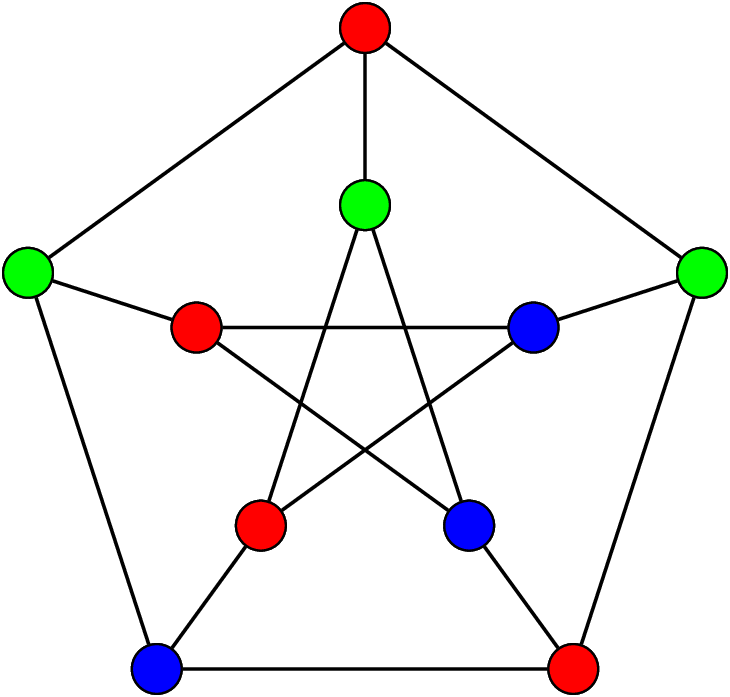
\includegraphics[width=0.8\textwidth]{petersenov_graf_barvanje} % first figure itself
        	\caption{Primer barvanja s $3$ barvami}
    	\end{minipage}\hfill
    	\begin{minipage}{0.45\textwidth}
       	 \centering
        	 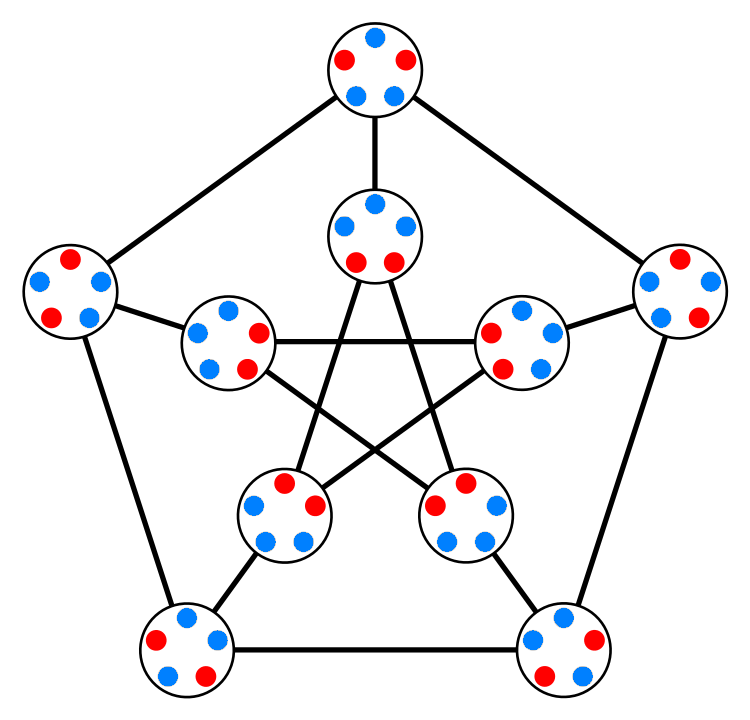
\includegraphics[width=0.8\textwidth]{petersenov_graf_mnozice} % second figure itself
       	 \caption{Prikaz povezav med disjunktnimi množicami}
    	\end{minipage}
\end{figure}

\end{frame}

%%%%

\begin{frame}{Kneserjeva domneva}

\begin{izrek}[Kneser]
Za kromatično število Kneserjevega grafa velja
$$\chi(K(2k+d,k)) = d+2.$$
\end{izrek}

\pause

\begin{izrek}[Ekvivalentno]
Če družino $k$-elementnih podmnožic množice $\{1, 2, \ldots, 2k+d\}$ razdelimo na $d+1$ razredov,  $V = V_1 \sqcup V_2 \sqcup \ldots \sqcup V_{d+1}$, potem obstaja $i$, da $V_i$ vsebuje par $k$-elementnih disjunktnih množic $A$ in $B$.
\end{izrek}

\end{frame}

%%%%

\begin{frame}{Potrebovali bomo:}

\begin{izrek}[Borsuk-Ulam]
Za vsako zvezno preslikavo $f:S^d \rightarrow \mathbb{R}^d$, z $d$-sfere v $d$-prostor, obstajata antipodni točki $x^*$ in $-x^*$, ki ju $f$ slika v isto točko, torej $f(x^*)=f(-x^*)$.
\end{izrek}

\begin{izrek}[Lyusternik-Shnirel'man]
Če je $d$-sfera $S^d$ pokrita z $d+1$ množicami,
$$S^d = U_1 \cup U_2 \cup \ldots \cup U_d \cup U_{d+1},$$
tako, da so vse izmed prvih $d$ množic $U_1, U_2, \ldots, U_d$ bodisi odprte bodisi zaprte, potem ena izmed $d+1$ množic vsebuje par antipodnih točk $x^*$ in $-x^*$.
\end{izrek}

\end{frame}

\end{document}